\section{Methodology}

\subsection{A Model of Suboptimality}
\todo{Sabah has the modify token}
The model suggests how some factors may impact the prevalence of
suboptimality. (In preliminary investigation, we have seen that
different queries are suboptimal in different DBMSes, and so it is
more productive to focus on the prevalence of suboptimality than on
the harder, and perhaps less illuminative, task of predicting which
individual queries produce suboptimal plans.) We present our model in
a hierarchical manner such that the dependencies among the components
can be directly revealed. We partition the factors in our model into
two categories, namely external and internal factors. ``Query
complexity'' is thus an external factor, in that they are not part of
the query optimizer. We can manipulate the external factors in the
experiment. Query complexity includes such factors as the number of
correlation names in the from clause, the presence of aggregates, the
number of self joins. The number of correlation names in the from
clause and the presence of aggregates will weakly influence
suboptimality directly. Instead, all the Query complexity
instantiations will influence suboptimality indirectly by influencing
plan space complexity. The number of correlation names in the from
clause will exponentially influence plan space complexity. The
presence of aggregates will linearly influence plan space complexity.
The number of self joins will negatively correlate with plan space
complexity. Structure of the tables used by the queries is another
external factor called ``Schema complexity''. Schema complexity
include factors like presence of primary keys and indexes.

[Is the sentence below accurate?]
Presence of primary keys, or indexes if present on columns involved in
the join condition between tables involved in a query, will reduce the
plan space complexity and thus inderectly reduce suboptimality present
in the query. [What is the function of the relationship between
presence of indexes and CEPS / Suboptimality]

Concerning the internal factors, some are independent variables, which
we can control, and some are {\em latent variables}, which are derived
from independent variables or which are internal to the optimizer. The
number of aggregates is an independent variable.

One of the central causal factors of this model is the optimizer
complexity. The model states that if the optimizer is very complex,
i.e., if the optimizer has to contend with a large number
of available operators, that will also increase the number of
interactions, and thus the
prevalence of suboptimal queries.

As we cannot observe the plan space complexity of the optimizer
directly, we include in the model other components, which may, from
different angles, indirectly help us understand the effects of the
complexity of the optimizer. Given a particular query, its measurable
complexity will impact the total number of candidate plans considered
by the optimizer. However, this latter factor is not directly
observable, again, especially for propriety systems. However, we {\em
can} measure the number of plans actually generated by the optimizer
when presented with different
cardinalities of the underlying tables. We term this set of plans
actually generated the
``effective plan space'' and the number of such plans, the
``cardinality of the effective plan
space,'' or {\em CEPS}. The model states a correlation between the
latent variable of the number
of plans considered and the measurable dependent variable of CEPS. The
model also states a
positive correlation between the number of operators available in the
DBMS and plan space
complexity. Another feature of the model is the positive correlation
between the number of
operators available in the DBMS and the number of operators observed
for each functionality. Only a subset of the physical operators
available will actually be considered depending on the
presence of a particular functionality (such as join) in the query.

We have just {\em described} how suboptimality might arise, through a
theory and its elaborated
model. We now discuss {\em prediction}.
How might we test such a theory? We hypothesize from our model that as
the optimizer becomes increasingly complex, more occurrences of
suboptimality will be observed, because of such unintended
interactions. Similarly, with a more simplistic optimizer, we
hypothesize that there will be fewer unanticipated interactions, and
so less suboptimality would be present. We predict that one source of
the suboptimality is the designer's focus on correctness and
performance, making it difficult to predict subtle interactions
between components of the optimizer. Later we explore the
ramifications of this hypothesis, finding support for our proposed
model.

\todo{Questions:}
1. I presume the following should go in section 1/ 4, since they are
related to how we
operationalized / tested hypotheses
- heuristic nature of some DBMSes
- Daemons and how we controlled for them

2. Do we still think that the different components of query
complexity, schema complexity and
optimizer complexity will influence suboptimality through CEPS? If so,
why didn't we see the
relationship last time? Or is the relationship between the independent
variables through cost
model accuracy (or some other factor) that we haven't operationalized yet?

3. How does primary keys / indexes impact suboptimality?


\todo{ operationalization def, high level}
Once a particular query is determined to be suboptimal, the obvious
next step would be to look at the code of the query optimizer (if
indeed the code is even available) and alter it in some way so that it
to reduce suboptimality. What we have done instead is to approach this
phenomenon from a scientific perspective, attempting to move to the
right on the $x$ axis of Figure~\ref{fig:empirical}, by developing a
simple predictive model of suboptimality, shown in
Figure~\ref{fig:model}.

The purpose of query optimization is to generate optimal plans.  So
why would suboptimality occur in the first place? Query optimizers are
highly complex, comprised of tens of thousands of lines of code. There
are several reasons for this complexity. First, an optimizer must
contend with the richness of the query language, SQL, whose definition
requires about 2000 pages~\cite{SQL2008}, with a multiple of
linguistic features. Second, an optimizer must content with the
richness of the physical operators available to it. DBMSes have a
range of algorithms available to evaluate each of many algebraic
operators. Third, the optimizer must contend with an exponential
number of query evaluation plans. Kabra and DeWitt~\cite{kabra98}
identify several other sources of complexity: inaccurate statistics on
the underlying tables and insufficient information about the runtime
system: ``amount of available resources (especially memory), the load
on the system, and the values of host language
variables.''~(page~106). They also mention user-defined data types,
methods, and operators allowed by the newer object-relational
systems~\cite{Melton03}. Thus, the task of optimization is very
complex, with the result that the optimizers themselves consist of a
collection of ``components,'' that is, the rules or heuristics that it
uses during optimization, with each of these components being itself
complex.

Our theory, which we will investigate in some detail and which is the
basis for our predictive model, is that suboptimality is due in part
to the complexity of the optimizer and concomitant unanticipated
interactions between the different components used within the 
optimizer.  We argue that with the proliferation of concerns and
variability that an optimizer must contend with, it is extremely
difficult to ensure that for an arbitrary query that the optimizer
will {\em always} pick the right plan. The components of the optimizer
are all interacting with each other; our theory implicate these {\em
interactions} as one source of suboptimality.

The model of Figure~\ref{fig:model} suggests how some factors may
impact the prevalence of suboptimality. (In preliminary investigation,
we have seen that different queries are suboptimal in different
DBMSes, and so it is more productive to focus on the prevalence of
suboptimality than on the harder, and perhaps less illuminative, task
of predicting which individual queries produce suboptimal plans.) We
present our model in a hierarchical manner such that the dependencies
among the components can be directly revealed. We partition the
factors in our model into two categories, namely external and internal
factors. ``Query complexity'' is thus an external factor, in that it is 
not part of the query optimizer. We can manipulate the external 
factors in the experiment. Query complexity includes such factors as
the number of correlation names in the from clause, the presence of
aggregates, the number of self joins. The number of correlation names
in the from clause and the presence of aggregates will weakly
influence suboptimality directly. Instead, all the Query complexity
instantiations will influence suboptimality indirectly by influencing
plan space complexity. The number of correlation names in the from
clause will exponentially influence plan space complexity. The
presence of aggregates will linearly influence plan space complexity.
The number of self joins will negatively correlate with plan space
complexity.
Therefore, our hypotheses with respect to the impact of Query Complexity are
Hypothesis 1: The number of correlation names will exponentially influence
Plan space complexity.
Hypothesis 2: The presence of aggregates will linearly influence plan space
complexity.
Hypothesis 3: The number of self joins will negatively correlate with
plan space complexity. 

Concerning the internal factors, some are independent variables, which
we can control, and some are {\em latent variables}, which are derived
from independent variables or which are internal to the optimizer. The
number of aggregates is an independent variable.

One of the central causal factors of this model is the optimizer
complexity. The model states that if the optimizer is very complex,
i.e., if the optimizer has to contend with a large number of available
operators, that will also increase the number of interactions, and
thus the prevalence of suboptimal queries.
Hypothesis 4: As the number of operators increase, the prevalence of suboptimality will increase.

As we cannot observe the plan space complexity of the optimizer
directly, we include in the model other components, which may, from
different angles, indirectly help us understand the effects of the
complexity of the optimizer. Given a particular query, its measurable
complexity will impact the total number of candidate plans considered
by the optimizer. However, this latter factor is not directly
observable, again, especially for propriety systems. However, we {\em
can} measure the number of plans actually generated by the optimizer
when presented with different cardinalities of the underlying tables.
We term this set of plans actually generated the ``effective plan
space'' and the number of such plans, the ``cardinality of the
effective plan space,'' or {\em CEPS}. The model states a correlation
between the latent variable of the number of plans considered and the
measurable dependent variable of CEPS. The model also states a
positive correlation between the number of operators available in the
DBMS and plan space complexity. Another feature of the model is the
positive correlation between the number of operators available in the
DBMS and the number of operators observed for each functionality. Only
a subset of the physical operators available will actually be
considered depending on the presence of a particular functionality
(such as join) in the query.
Hypothesis 4: Plan space complexity (CEPS) linearly influences suboptimality.

\todo{Add a few sentences about number of operators observed across functionality. }
The types of functionality involved vary based on the type of SQL query. 
For each functionality, the DBMS may include multiple different physical operators
to implement the functionality. The main
types of functionality included in this study involve joins, and aggregates. 
Within joins, we also looked at the impact of self joins. Optimizers have
different operators for each functionality. For example, if the query did 
not involve joins, none of the join operators would be considered and thus
they would not contribute to the complexity for that query. Although we cannot
extract the operators that were considered for proprietary DBMSes. However, 
we can approximate this by observing the operators that were selected 
across different queries sharing functionality. And, that is what we did
to measure operators.

In the characterization of the $x$ axis of Figure~\ref{fig:empirical}
of empirical generalization, we have just {\em described} how
suboptimality might arise, through a theory and its elaborated model.
We now need to move right on that axis, to {\em prediction}.

How might we test such a theory? We hypothesize from our model that as
the optimizer becomes increasingly complex, more occurrences of
suboptimality will be observed, because of such unintended
interactions. Similarly, with a more simplistic optimizer, we
hypothesize that there will be fewer unanticipated interactions, and
so less suboptimality would be present. We predict that one source of
the suboptimality is the designer's focus on correctness and
performance, making it difficult to predict subtle interactions
between components of the optimizer. Later we explore the
ramifications of this hypothesis, finding support for our proposed
model.
\todo{Also add details why our model is necessary before examining data
skew, indexes, etc. }



\subsection{Detecting Suboptimality}
\todo{Get adjacent from operationalization.
 assumptions: time query repeatable, timing monotonic}

\todo{Rick has modify token: merge these two sections.}
\todo{ original adjacent scenario, change points, monotonicity}

How might such behavior be observed? We have developed a system, \azdb, that
allows us to perform experiments to study this phenomenon of suboptimality.
\azdb\ can externally modify data
dictionary statistics for tables and columns, thereby allowing the DBMS to
generate different plans for a given query.
\hbox{\azdb} then presents queries to the DBMS while varying
the statistics, in particular the cardinality of one of the tables,
requesting in each case the evaluation plan chosen by the DBMS.
This is done using the
{\tt EXPLAIN} SQL facility available in modern DBMSes. We can thus compare
the performance (execution time) of various plans for the query, to identify those
situations when the wrong plan was chosen, when in fact there was a
different plan that was semantically equivalent to the chosen plan (that is,
yielded the identical result) but which ran faster.

\begin{figure*}[tb]
\centering
%originally 30pc
\epsfig{figure=figures/model.eps,width=30pc}
\caption{Predictive Model of Suboptimality\label{fig:model}}
\end{figure*}

\comment{\azdb\ modifies the cardinality statistics to produce multiple execution
plans for a given query. For one of the DBMSes, we can modify the stored
table statistics directly. For the other DBMSes, we had to do so indirectly,
by varying the size of the table and running the optimizer on tables of
different size. As \azdb\ varies the cardinality statistics of tables, it
collects all the plans that the optimizer felt were appropriate for that
query.  After \azdb\ gathers the plans, it then executes each plan on the
original table(s), to determine which plan was actually the best, of the
plans generated by the optimizer. 
}
It is important to note that all of this manipulation can be done {\em
  outside} the DBMS. For proprietary systems we do not have access to the
internal code. We don't know ({\em can't} know) all the plans that were
considered, nor the details of how the plans are selected. But such access
is not needed; indeed, to be able to study a phenomenon across many DBMSes,
such access is not practical. But by designing the experiment to examine
the plans that the DBMS actually produces, and thus to examine phenomena
that can be externally visible, we can obtain valuable insights into general
classes of computational artifacts. Our ultimate goal is to make statements
that hold across cost-based optimizers in general, thereby moving up the
$y$-axis of Figure~\ref{fig:empirical}.




\subsection{Measuring Query Execution Time}\label{sec:subopt}
\todo{Young has modify token}
\todo{phantom...}
In order to quantitatively examine the effects of suboptimality, we need to
measure the execution time of each plan of each query.

In this scenario, sub-optimality is defined by the existence
of a plan, produced at a non-actual table cardinality, that runs with a
shorter elapsed-time than the ``optimal'' plan chosen and executed at the
(same) actual cardinality. {\tt stepA} populates the variable table. {\tt
  stepB} times the execution plan for the actual table size and returns
statistics on that execution. {\tt stepC} changes the cardinality statistics
of the variable table and always returns true. {\tt stepD} times the plan
for the specified cardinality, which was set by the previous step.

\todo{Rick: Could you please read through this paragraph. }
\todo{Extract text about change points and modify for adjacent. }
\todo{Talk about adjacent and why we measured it and how. } 
The ``optimal'' plan is the plan chosen at the actual cardinality. It may 
be chosen at other cardinalities too. 
The ``Adjacent'' scenario is used when a DBMS does not allow the statistics to
be changed. This scenario simply executes the query by successively changing
the cardinality of the varying table, by starting at the maximum and
deleting tuples. Periodically (every 10K tuples deleted), the query is
optimized, and run whenever the plan changes. In this scenario, a more
conservative definition of suboptimality is used. After the identification of the occurrences of change points, i.e., when the optimized plan chosen changes, 
the running time for each optimized plan is compared to the ``optimal'' plan that is 
closest to it at a lower cardinality. Suboptimality is defined
by the existence of a plan, produced with a larger varying table table
cardinality, that still runs with a shorter elapsed-time than the
``optimal'' plan chosen and executed.


We worked very hard to ensure the correctness and repeatability of the
execution time measurements. In developing \azdb, we encountered many sources
of DBMS variance for a given DBMS, a given query, and a given plan. Hence,
much of our effort was devoted to determining why a particular measurement
wasn't repeatable, and then eliminating that variance. We were hampered by
the fact that DBMS documentation is generally quite incomplete on this
subject\c2j{}{, and by the fact that our solutions were quite idiosyncratic to the
DBMS involved}. We were also challenged by the fact that we had to be able to
solve the problem only through the facilities available to JDBC: we could
not make any internal changes to the DBMS.

The presence of flutter, sometimes prevalent, indicates that the optimizer
appears to not be making good choices as the cardinality estimate is less
and less accurate. We saw that graphically in Figure~\ref{fig:query769}, as
the query plan fluttered between Plans 2 and 4 for a wide range of
cardinality estimation error for Query~769.

Perhaps the optimizer is not even making a good choice when the estimate is
entirely accurate. Such was the case for Query~769: that plan was not the
fastest of the five plans, having an execution time that was almost the same 
as the worst plan, Plan~2.

The presence of flutter indicates the optimizer is having a hard time
picking a plan. It seems possible that in such situations the optimizer may
pick the wrong plan.

Because we can execute the various plans generated by the optimizer on the
actual cardinality, we can see whether the optimizer in fact picked the best
plan, out of the options in the effective plan space. We ran the same 600 queries 
with timing enabled on DBMS {\bf A}.

It is interesting to see how far off the optimizer
was in such cases. Figure~\ref{fig:diff} shows the execution time difference by percentage
between the chosen plan and the fastest plan, shown ordered by
percentage. Our results show that most of the sub-optimal queries have chosen plans 
that are several times slower that the fastest plan.

\c2j{We obtained different plans for each query by varying the cardinality
  statistics of one of the tables; these statistics are used by the optimizer.}{We obtained different plans for each query by varying the cardinality
of one experiment table, which we called the ``variable table'' in our
experiments. We developed two approaches to perform the tests.

In the first approach, we fixed the actual size of the variable table. However,
we altered the table statistics stored in the DBMS system catalogs; these
statistics are used by the optimizer.In practice, 
only one DBMS out of the three allowed us to manipulate the 
table statistics through the JDBC API. Thus we present results on 
query plan execution time using such approach only for DBMS~{\bf A}.}
The purpose of this approach is to find out whether there exists a plan
that is better than the plan the DBMS chose as the ``optimal one'' with
accurate cardinality, given that these plans are run on the same set of
tables.

\c2j{Utilizing JDBC to manipulate independent variables from outside the
  DBMS allows us to empirically generalize by moving up the $y$ axis of
  Figure~\ref{fig:empirical}, from one system to several systems and then to
  a general theory. However, as we discuss in detail shortly, obtaining {\em
    repeatable} and {\em accurate} timings of database queries was
  unexpectedly difficult. So in this paper we report experiments over just
  one DBMS. We plan to generalize the results and the tests over a range of
  DBMSes, once we are able to obtain accurate, repeatable timing results for
  each. We don't reveal the identity of the DBMS we studied, for two reasons. First, commercial DBMSes
include in their user agreements requirements not to release 
performance data. This is detrimental to science, but we have no choice but
to live with that restriction. However, in some sense the specific DBMS
doesn't matter, as we are studying phenomena about cost-based optimizers
{\em in general}, and so are interested in making statements that apply to
all the experimental subjects in our study.}{In the second approach, we varied the cardinality of the variable
  table by actually deleting tuples from it. To ensure the correctness of
  the plan generation and thus time measurements, we performed an ``ANALYZE
  TABLE`` function to force the DBMS to update the table's new statistics to
  be accurate. The purpose of this approach is find whether there exists a
  plan that runs faster with a larger table than a different plan that is
  executed on a smaller table.}

\shorten{\begin{figure*}[htb]
\begin{small}
\begin{verbatim}
<experiment name="X" scenario="veryCardinalityStats" dbms="...">

    <dataDefinition name="ft">
      <table name="HT1" cardinality="1000000">
        <column name="id1" dataType="number" dataLength="10" dataGenerationType="sequential"
                distributionMinimum="0" distributionMaximum="1000000" inPrimaryKey="false"/>
        <column name="id2" dataType="number" dataLength="10" dataGenerationType="random"
                distributionMinimum="0" distributionMaximum="1000000" inPrimaryKey="false"/>
        <column name="id3" dataType="number" dataLength="10" dataGenerationType="random"
                distributionMinimum="0" distributionMaximum="1000000" inPrimaryKey="false"/>
        <column name="id4" dataType="number" dataLength="10" dataGenerationType="random"
                distributionMinimum="0" distributionMaximum="1000000" inPrimaryKey="false"/>
      </table>
      <table name="HT2" cardinality="1000000"> (same as above) </table>
      <table name="HT3" cardinality="1000000"> (same as above) </table>
      <table name="HT4" cardinality="1000000"> (same as above) </table>
    </dataDefinition>
   
    <tableConfiguration>
      <variableTableSet searchMethod="linear" searchGranularity="10000"> <table name="HT1" seed="1999">
          <cardinality hypotheticalMinimum="1" hypotheticalMaximum="2000000"/>
        </table>
      </variableTableSet>
      <fixedTableSet>
        <table name="HT2" seed="2999"> <cardinality hypothetical="actual"/> </table>
        <table name="HT3" seed="3999"> <cardinality hypothetical="actual"/> </table>
        <table name="HT4" seed="4999"> <cardinality hypothetical="actual"/> </table>
      </fixedTableSet>
    </tableConfiguration>

    <queryDefinition numberQueries="500" ...>
      <grammar>
        <select maxColumns="4"/>
        <from maxCorrNames="4" useDuplicates="true"/>
        <where cartesianPossible="false" maxIsAbsolute="true" maxPredicates="0" complexUsePercentage="100">
          <binaryOperators> <operator symbol="="/> </binaryOperators>
          <binaryLogicalOperators> <operator symbol="AND"/> </binaryLogicalOperators>
          <unaryLogicalOperators> <operator symbol="NOT" usePercentage="0"/> </unaryLogicalOperators>
        </where>
      </grammar>
    </queryDefinition>

</experiment>
\end{verbatim}
\end{small}
\vspace*{-4ex}\caption{The XML specification of the experiment\label{fig:expspec}}
\end{figure*}
}

\subsubsection{Single Execution Time Measurement}\label{sec:qe_time}

\begin{figure}[th]\centering
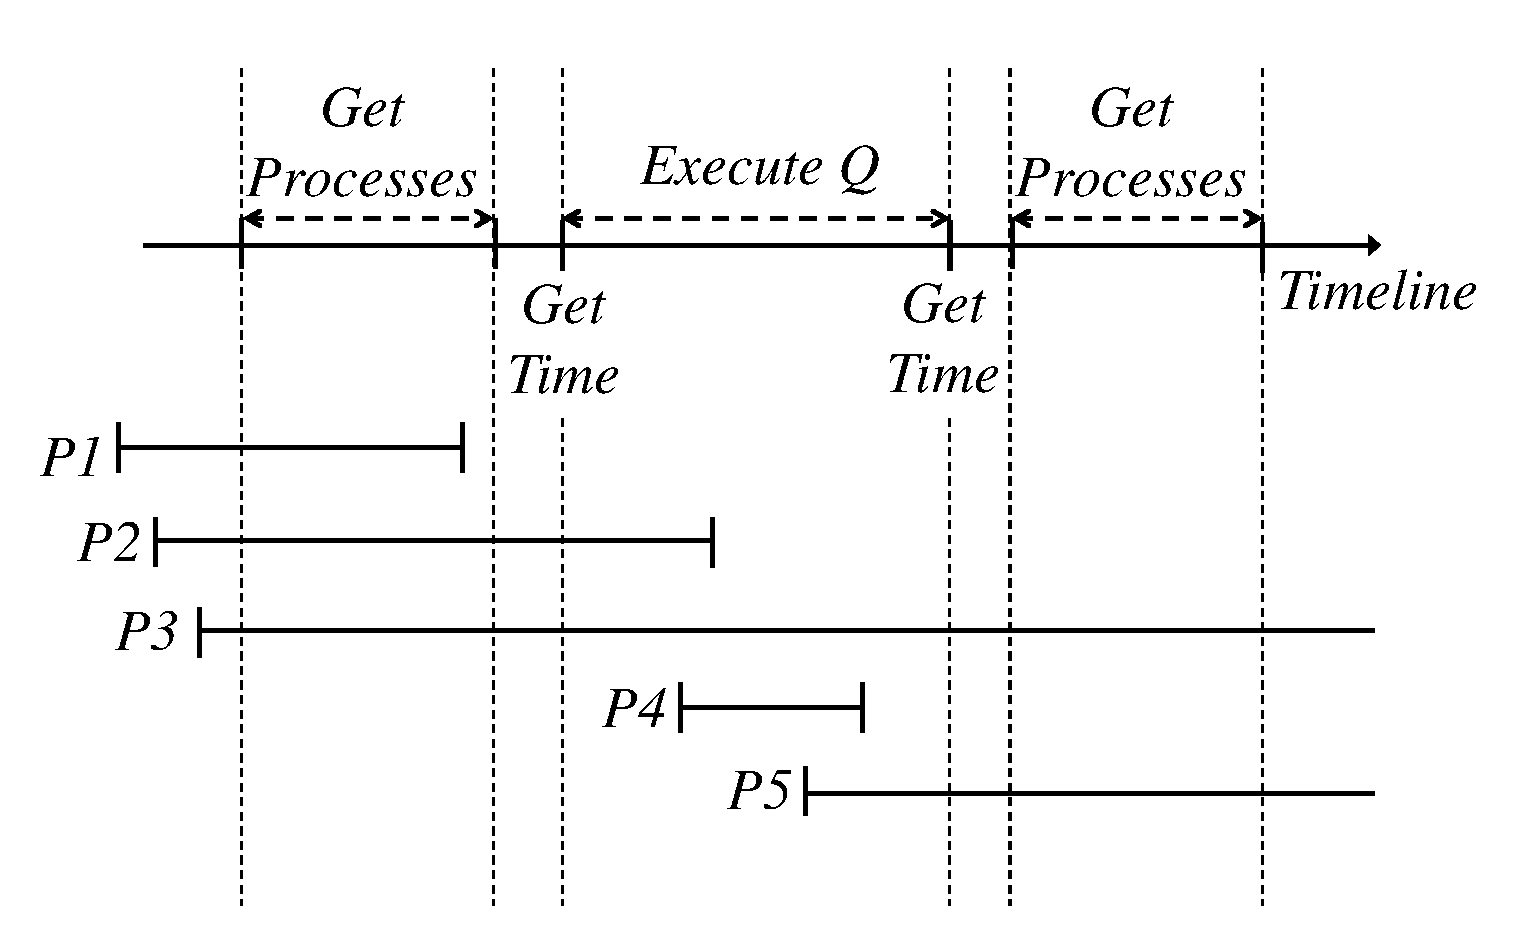
\includegraphics[width=0.50\textwidth]{figures/time_measurement.eps}
\caption{Processes influencing query execution\label{fig:timing}}
\end{figure}

In this section we discuss how we measure query execution time. 
As illustrated in Figure~\ref{fig:timing}, 
we first get all running processes before executing 
a query $Q$. 
Then timer for $Q$ gets started, and it is stopped after $Q$ gets 
executed. 
The execution time for $Q$ is measured by the time difference, and 
we finally finish single query execution by examining running 
processes right after the execution. 

Now let us examine how other processes may influence query execution. 
Assume that all the processes below are not relevant to DBMS processes.
Before timing $Q$, processes $P$1, $P$2 and $P$3 are recorded into 
a map $M$1. 
Another map $M$2, on the contrary, keeps processes $P$3 and $P$5 
captured after the timing. 
For each recorded process, the maps $M$1 and $M$2 keep 
$<$process id (pid), \{process name, minimum/major faults, 
cpu/system times\}$>$. 
The cpu and system times are considered for the subtraction. 
The process information can be achieved by iterating 
{\tt /proc/\{pid\}/stat} associated with each process. 

By comparing $M$1 and $M$2, we easily know that $P$3 and $P$5 affected 
$Q$'s execution; thus, the time spent on $P$3 and $P$5 are subtracted from 
the measured query execution time. 
$P$1 and $P$2 that do not appear in $M$2 must have stopped 
before or during the query execution, respectively. 
We cannot determine whether the query execution is affected by 
these stopped processes. 
For instance, $P$2 is explicitly involved with the execution whereas 
$P$1 not. 
What we can know is that regarding the execution, there were stopped 
processes, such as $P$1 and $P$2, as a result of comparison with 
$M$1 and $M$2. 
This execution, therefore, will be thrown out due to the stopped ones. 

Note that $P$4 is a {\em phantom} process, since it does appear 
in neither $M$1 nor $M$2. 
The existence of phantom process can be known by comparing 
the number of processes from {\tt /proc/stat} before and after execution.
Like stopped processes, we throw out any execution with a phantom process, 
considering measurement accuracy.

\begin{figure}[t]
\begin{center}
\begin{algorithmic}
{\bf Algorithm} timeSingleQueryExecution($i$, $q$, \\
						\hspace{44.0mm}$exPlan$, $card$):
\STATE $plan$ $\leftarrow$ get(Prepared)QueryPlan($q$)
\IF{$plan$ $\neq$ $exPlan$}
	\STATE Error: two different plans are observed \\ 
	at the same cardinality. \\
\ENDIF
\STATE Flush disk drive/OS/DBMS caches. \\
\STATE $M1$ $\leftarrow$ $extractAllRunningProcs$() \\
\STATE $startTime$ $\leftarrow$ $getCurrTimeMills$() \\
\STATE $executeQuery$($q$) \\ 
\STATE $endTime$ $\leftarrow$ $getCurrTimeMills$() \\	
\STATE $execTime$ $\leftarrow$ $endTime$ - $startTime$ \\	
\STATE $M2$ $\leftarrow$ $extractAllRunningProcs$() \\
\STATE $procDiff$ $\leftarrow$ $diff$($M1$, $M2$) \\	
\STATE RecordQueryExecution($i$, $q$, $card$, \\ 
			\hspace{34.0mm}$execTime$, $procDiff$) \\
\end{algorithmic}
\caption{Timing single query excution\label{alg:timing}}
\end{center}
\end{figure}



\section{Repeatability}
We ensure the validity of our experiment results examining the
{\em repeatability} of our experiments. 
The repeatability study focuses on three factors, namely
{\em data repeatability}, {\em within-run repeatability},
and {\em across-run repeatability}, respectively.

First, repeatability is examined within data. Although the data 
that is populated for experiment tables are randomly generated, we ensure the
same numbers are generated each time.
Second, the query plans produced at the same cardinality for the same query
should be identical. Finally, as the cardinality of the variable-table
reduces, change points, where a different plan is detected, are identified. 
The experiment is repeatable if the same set of change points, which appears 
at the same cardinalities across multiple experiment runs, can be identified. 

\shorten{
We use the following query $Q$ as an example to explain repeatability.

\begin{center}
\begin{tabular}{rl}
$Q$:	& {\tt SELECT t2.id4, t3.id1} \\
		& {\tt FROM HT2 t3, HT1 t0, HT4 t2, HT3 t1} \\
		& {\tt WHERE (t3.id4=t0.id1 AND }  \\
		& {\tt t0.id1=t2.id1 AND t2.id1=t1.id4)} \\
\end{tabular}
\end{center}
}
\shorten{
We first obtain a plan at 1M rows of {\tt HT1} (1M plan). 
Then, we find different plans, deleting the end of 10K rows 
from {\tt HT1} initially loaded with 2M rows (max) 
until the minimum cardinality which is 1M rows. 
All change points are also recorded with the plans.

In the second pass, $Q$ gets executed at all change points including 
the first 1M rows. 
We double-check whether the plan found at the change point is equal to one 
obtained at the time of execution. 
The executions for $Q$ are later used for telling the suboptimality of $Q$ 
by comparing the execution time of the 1M plan with that of other plans.

Interestingly, what we found was that in the first pass we happened to 
observe two different plans at 1M rows of {\tt HT1}. 
That is, the plans at 1M rows were inconsistent with each other 
even though all the involved tables' cardinalities were the same. 
}

\shorten{
The repeatability issue is initially raised from an experimental scenario, 
termed {\em Adjacent}, which studies query sub-optimality. 
(For more details about query suboptimality, please refer to 
Section~\ref{suboptimality}.)
The scenario includes data definition, query definition, and 
query plan detection and execution strategy. 
By data definition, we populate a few tables with fixed cardinality, 
saying 1M rows, and use a variable-table to get cardinality changing. 
Queries can be generated or pre-defined by query definition. 
For instance, let us consider the following query $Q$.}

This query involves four distinct tables, namely {\tt HT1}, {\tt HT2},
{\tt HT3}, and {\tt HT4}, which are all configured with the same sets of
columns, namely ({\tt id1}$\sim${\tt id4}). These four tables participate
in three joins, each joining a distinct pair of tables.
Tables {\tt HT2}, {\tt HT3}, and {\tt HT4} have the same fixed cardinality,
which is 1M rows. We term these tables the {\em fixed}-tables.
On the other hand, {\tt HT1} is termed a {\em variable}-table in that we
vary its cardinality from 2M rows down to 10K rows, at a step of 10K rows
each time.

\subsection{Data Repeatability}
To populate these tables, we utilize a random number generator. The values
for column {\tt id1} across the four tables are sequentially assigned.
The values for the other columns are populated by the generator. We control
the seed for the number generation such that the produced sequence of
``random'' numbers are identical each time. To change the cardinality of
the variable-table, we populate this table to the maximal cardinality,
which is 2M rows, and then {\tt DELETE} from the end of the table 10K rows
at a time.

\subsection{Within-Run Repeatability}
To study suboptimality in query evaluation, we define an experiment scenario
to carry out the experiment in an automated and structured fashion.
The scenario contains two execution stages.
In the first stage, we initially populate the variable table to have 1M rows,
which is the same to the fixed tables. We utilize the {\tt EXPLAIN} command
to produce the execution plan for $Q$ and then execute the query to measure
the running time. This measurement is used as a reference point for further
study.
We then re-populate the variable table to the maximal of 2M rows, and we delete
10K rows from the end of the table each time and call {\tt EXPLAIN} to
collect the plans. As the cardinality is reduced, if the newly generated plan
is different from the previous one, we note the current cardinality as a
{\em change point} and we store the cardinality as well as the plan. At the
end of the first stage, we usually collect a list of change points.

In the second stage, we re-populate the variable table to the maximal
cardinality again. According to the list of change points, we can directly
delete a number of rows from the variable table to achieve the target
cardinality at which a change point was found in the previous stage.
We run the query at the point to measure the running time. To ensure
that the current query execution utilizes the same time as the corresponding
change point, we compare the two plans.

An interesting observation is that sometimes in the two stages, a change
point is identified at cardinality 1M. The occurring plan at this change point
is different from the the reference plan initially generated. The reason
is that by deleting rows from a table, the deleted rows are simply flagged
without being physically removed. This leads to the issue that the number of
occupied pages, which is a factor considered by the cost model employed by
the optimizers, does not tightly correlate with the number of rows in the
table.

\shorten{
One of the reasons we speculated was that a way of setting the cardinality 
for the variable table might cause the optimizer to choose different 
plans in spite of the same cardinalities. 
To vary the cardinality of {\tt HT1}, a table with the same definition 
as {\tt HT1}, called {\tt max$\_$HT1}, is populated to the max cardinality, 
2M rows. 
To get the first 1M plan, the 1M rows of {\tt HT1} were copied from {\tt max$\_$HT1}. 
On the contrary, the second 1M plan was acquired due to the 10K-row-deletion. 

To see whether the plan difference, or unrepeatability reappeared even after 
making cardinality by a consistent method, 
we also tried other variety of scenarios: {\it deleteTop10K}, {\it doubleTriple}, 
{\it copy1M}. 
In {\it deleteTop10K} scenario, {\tt HT1} is first loaded with 2M rows 
by the max table copy, and 10K rows from {\tt HT1} are incrementally 
deleted until 1M rows. 
A 1M plan is eventually acquired at the minimum cardinality as before. 
We repeat these steps so that both of the 1M plans can be compared 
for repeatability check. 

{\it DoubleTriple} scenario basically extends {\it deleteTop10K}. 
Four plans are obtained by running {\tt deleteTop10K} scenario twice. 
Thereafter, instead of the incremental deletion, we get a 1M plan right after 
copying 1M rows into {\tt HT1} from the max table as before. 
By repeating this, the total six plans are obtained. 
We ensure repeatability by checking whether all of the six 1M plans are identical. 
}

To address the issue that the number of pages and the number of rows are not
correlated, we designed a new scenario, essentially with a different
cardinality-varying mechanism. We term this new scenario {\em copy1M}.
Unlike deleting rows, the alternative mechanism creates a new table and
utilizing the {\tt SELECT ... INTO ...} command to populate the newly created
table to the target cardinality. This approach effectively ensures that
the cardinality of the table is coupled with the number of pages the table
occupies.

\subsection{Across-Run Repeatability}
While the within-run repeatability is ensured, we run each experiment multiple
times to collect running time samples for statistical analysis. A change point
can be uniquely identified by the query ID and the cardinality value within
a run. Hence by grouping the change points with the same query ID and
cardinality value across multiple runs, should the samples be correctly
collected for each change point.

Nonetheless, we observed that for the same query, different sets of change
points are found for various runs. We utilized one DBMS to conduct a simple
test, that is to invoke the {\tt EXPLAIN} facility with the same query
at different times, which was often one minute apart or hours apart. The
underlying tables were of course not changed whatsoever. We found that
the produced plans at various times could actually be different even though
the tables stay unchanged. We concluded that this plan inconsistency issue
was due to the randomness introduced by the heuristics adopted by
DBMSes to compute the table stats.

Given that it is difficult to ensure the across-run repeatability,
we altered the approach to collecting multiple running-time samples.
Instead of execute multiple runs for each experiment, each plan, once
identified, is executed multiple times such that the samples are guaranteed
to be collected on the same plan.

In fact,\todo{is this true? I don't have facts to back this up...} the
within-run repeatability was sometimes violated due to a similar
reason. In the adjacent scenario, two stages (passes) are made to identify
and execute query plans, respectively. However, the plan produced in the
second pass could be different from the first pass.

To address the randomness caused by the optimizer, we restrict that
the optimizer only produces plan once for the same query at the same
cardinality. We term this new approach {\em onePass}. The resulting
new scenario is termed accordingly. In this scenario, instead of making
two passes of varying the cardinality of the variable table, the cardinality
is only varied once such that once a change point is identified, the generated
plan is executed multiple times. This scenario finally resolved the
repeatability violations in our experiments.
\todo{Do we talk about the two-table settings here?}


\subsection{{\tt OnePass} Scenario}\label{sec:onepass}

In {\tt OnePass} Scenario, a query is studied for suboptimality by keeping track 
of the {\em states} on the variable-table. 
In other words, we locate different query plans at adjacent cardinalities 
defined by the {\em even} or {\em odd} states, 
and query executions are made at both of the states simultaneously, 
while decreasing the variable-table cardinality in one pass. 

Indeed, the adjacent cardinalities are not really called even and odd, 
but they are next to each other. 
They, thus, are simply separated by whether a given cardinality over 
granularity is even or odd. 
For instance, the even state will have 2M, 1.98M, 1.96M, $\cdots$, 1M cardinalities 
in order, while the odd state will take 1.99M, 1.97M, $\cdots$, 1.01M cardinalities 
(decremented by granularity (10K) from the even state's cardinality). 

Each state initializes its table(s) same as the variable-table(s). 
In addition, it has the {\em pre-compiled} query plan at its own cardinality 
so that the given query can be executed by the {\em prepared} plan at the cardinality 
without any compiling overhead.

While stepping down from the max to the min cardinality, 
if different query plans are observed at the even and odd states, 
then the prepared query execution at both states is made at the same time 
unless the query has been executed at the cardinality before. 
In this regard, for repeatability we time the same query up to 10 times. 
The timing results at each state are inserted into the labshelf for 
suboptimality analysis. 
For more details about timing single query execution, 
please refer to Section~\ref{sec:timing}.

\begin{figure}[t]
\begin{center}
\begin{algorithmic}
{\bf Algorithm} analyzeQuery($q$, $varTables$):
\STATE $evenState$.$initialize$($varTables$) \\
\STATE $oddState$.$initialize$($varTables$) \\
\FOR{$card$ = 2M to 1M by 10K}
	\IF{$\dfrac{card}{10K}$ is $even$}
		\STATE $evenState$.$card$ $\leftarrow$ $card$ \\
    	\STATE $evenState$.$plan$ $\leftarrow$ $evenState$.$getPreparedQueryPlan$($q$) \\
    \ELSE
 	    \STATE $oddState$.$card$ $\leftarrow$ $card$ \\
	    \STATE $oddState$.$plan$ $\leftarrow$ $oddState$.$getPreparedQueryPlan$($q$) \\
    \ENDIF
    \IF{($evenState$.$plan$ $\neq$ $oddState$.$plan$)}
		\IF{$\neg${$evenState$}.$isExecuted$()}
			\FOR{$i$ $\leftarrow$ 1 {\bf to} 10}
				\STATE $timeSingleQueryExecution$($i$, $q$,  \\
						\hspace{14.0mm}$evenState$.$plan$, $evenState$.$card$) \\
			\ENDFOR
		\ENDIF
		\IF{$\neg${$oddState$}.$isExecuted$()}
			\FOR{$i$ $\leftarrow$ 1 {\bf to} 10}
				\STATE $timeSingleQueryExecution$($i$, $q$,  \\
						\hspace{14.0mm}$oddState$.$plan$, $oddState$.$card$) \\	
			\ENDFOR
		\ENDIF
	\ENDIF
\ENDFOR 
\end{algorithmic}
\caption{Algorithm for Analyzing a Query by {\tt OnePass} Scenario\label{alg:onepass}}
\end{center}
\end{figure}


\subsection{Summary}
In summary, we learned various tricky situations where repeatability
could be violated during experiments and designed the one-pass scenario
to address these issues. Moreover, we experienced great variance in
running-time measurements due to system daemons and cron jobs. We had most
of the unnecessary processes turned off, which effectively reduce the
variance in measurements. We consider this also an effort to ensure the
repeatability for the experiments, in terms of running-time sample collection.

\todo{Young mentioned exhaustive before, but I now think it should go to the monotonicity section.}
\todo{Rick and Young agreed with Rui about this.}
\shorten{
We first applied these scenarios to DBMS A through E with a few runs of 100 queries. 
As a result, DBMSes A and B showed the repeatability for all queries. 
In particular, they were not affected by which of the above scenarios 
was run or how many times the scenario was run. 
On the contrary, the other DBMSes C, D and E failed to retain repeatability. 
They were sensitive to queries, runs and scenarios. 

As a last check, we also took advantage of CLI (Command-Line Interface) on 
the unrepeatable DBMSes in order to see directly the 1M plan without passing 
through the scenarios. 
DBMS C showed the same plan at a cardinality for a query at all times. 
However, the other two DBMSes D and E produced different plans for the same 
query at times.

The empirical observation about repeatability can be summarized as follows. 
Some heuristic algorithms may be exploited for the optimizers of DBMS 
D and E, which may affect the enumeration and decision of query plan. 
(To figure out this, we made several attempts to look for {\tt heuristic} keyword 
from the source code of DBMS D and E optimizers. 
However, it was not clear of where it was used.) 
DBMS C has relatively plenty of operators compared with other DBMSes, so 
its compatible operators may show up at different times, considering that plans 
built by such operators would have the same execution cost. 
In the meantime, DBMS A and B were repeatable.

Based on the observation from all the DBMSes, we eventually ensure 
repeatability (and monotonicity) by using {\tt exhaustive} scenario.
In {\tt exhaustive}, multiple query executions are made at each cardinality, 
varying the max cardinality to the min one; namely, for a query we get a plan 
and execute the query multiple times, saying 10, upon decreasing the cardinality. 
Instead of the incremental 10K-row-deletion, 
changing the cardinality is done by copying from the max table as many rows as needed 
so that all pages are in full with the rows. 
This setup allows us to check if any of the multiple executions produces 
different plans at the same cardinality (and see if the query execution 
times are monotonically decreasing as cardinality decreases). 
Each DBMS ran {\tt exhaustive} with a run of 10 queries, and it had 
no case such that different plans were detected at the same cardinality 
while a query got executed repeatedly.
}


%\subsection{Ensuring Monotonicity}
\todo{Sabah has modify token}


\subsection{Summary of Sub-Optimality}
\shorten{
In this paper we utilize a new methodology to ask new
questions about a mature topic, query optimization, in \hbox{order} to develop and
test a novel model and theory about when suboptimality arises, to
arrive at a new understanding of query optimization. This may later enable
new engineering approaches as well as a better understanding of the limits
of existing approaches.

\begin{figure}[bth]\centering
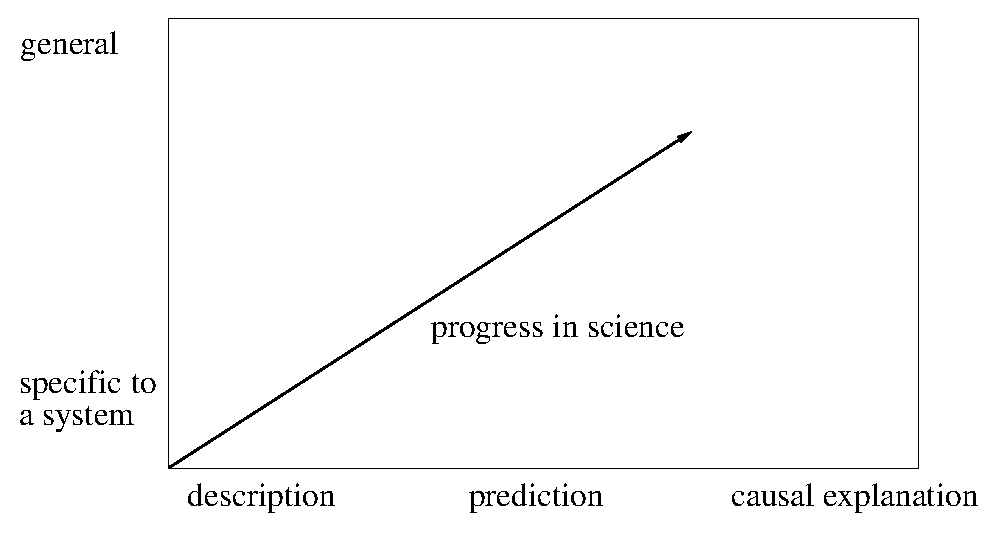
\includegraphics[width=0.50\textwidth]{figures/understanding.eps}
\caption{Empirical generalization ([3, page~5])\label{fig:empirical}}
\end{figure}

This paper utilizes {\em empirical
  generalization}, in which understanding proceeds along two conceptual
dimensions, as shown in Figure~\ref{fig:empirical}. As Cohen~\c2j{\cite{cohenbook}}{[1995]} has
articulated, science (in general, and this paper specifically) progresses
(in the figure, on the 
$y$-axis) from studies of a particular system (e.g, a particular database
query optimization algorithm in the context of a particular database
management system), through studies of a class of systems (e.g.,~a study
{\em across} several disparate DBMSs), to statements about computational
tools in general (e.g.,~a theory that holds for rule-based optimizers,
whether in DBMSs, AI systems, or compilers). This progression increases the
domain of applicability, and thus the generality, of a theory. Science also
progresses (in the figure, on the 
$x$-axis) from description of the phenomenon, to prediction, and eventually
through causal explanation, within an articulated, thoroughly-tested theory.
We seek the rather ambitious outcome of the articulation of a general theory
of suboptimality that applies to the entire class of DBMSes and which
provides causal explanation of suboptimality: when it will arise and why.

Note that this line of study is very different from conventional
approaches summarized above from the literature. We are trying to understand
cost-based query optimizers as a {\em general} class of computational artifacts,
to come up with insights and ultimately with predictive theories about how such
optimizers, again, as a general class, behave~\cite{davies}.}
